\documentclass[tikz,border=2mm]{standalone}
\usepackage[T1]{fontenc}
\usepackage[swedish,english]{babel}
\usepackage{tikz}
\usetikzlibrary{arrows,positioning}
\usepackage{pgfplots}
\usepackage{amsmath,mathtools}
\usepgfplotslibrary{fillbetween}
\begin{document}
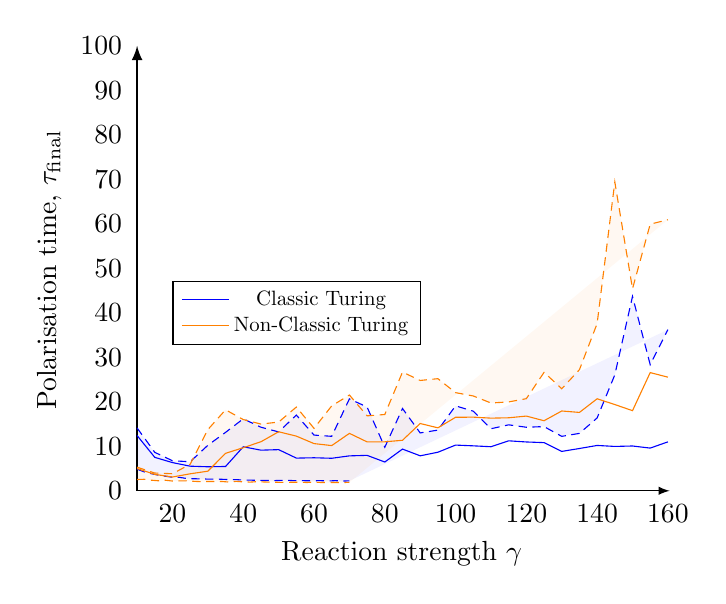
\begin{tikzpicture}
\begin{axis}[
    %hide axis,
    %axis lines* = left,
    %axis lines=left, xtick=\empty, ytick=\empty.
    axis line style={draw=none},
    tick style={draw=none},
    xticklabel style={yshift=-0.1mm},
    xmin = 8.5,
   xmax = 161,
    ymin = -0.75,
    ymax = 100,
    %grid=both,
    %xtick = {1,0.95,...,0.6},
    ytick = {0,10,...,100},    
    %xticklabels = {{zero},$\alpha$,$\varphi$},
   %xlabel style={at={(axis cs:0.61,7)},anchor=east,align=center},
    %ylabel style={at={(axis cs:1.00,35)},anchor=north,rotate=0},
	xlabel = {Reaction strength $\gamma$},
        ylabel = {Polarisation time, $\tau_{\textrm{final}}$},
    legend style={at={(axis cs:20,40)},anchor=west,cells={align=center},nodes={scale=0.75}},
    %x dir=reverse
    %legend entries = {Decreasing the inactivation rate $k_{-2}$}
]
%-------------------------------------------------------------------------------------------------
% AXES
\draw[->,-latex, thick] (axis cs: 10,0) -- (axis cs: 10,100); % y-axis
\draw[->,-latex] (axis cs: 10,0) -- (axis cs: 160.5,0); % x-axis
%-------------------------------------------------------------------------------------------------
%-------------------------------------------------------------------------------------------------
% Classical 
%-------------------------------------------------------------------------------------------------
\addplot[forget plot,densely dashed,color=blue,name path=UppolTimeClassical] coordinates {
		(10.0000	,	14.1177	)
		(15.0000	,	8.6423	)
		(20.0000	,	6.7462	)
		(25.0000	,	6.5300	)
		(30.0000	,	10.2303	)
		(35.0000	,	13.1299	)
		(40.0000	,	16.1730	)
		(45.0000	,	14.2878	)
		(50.0000	,	13.2351	)
		(55.0000	,	17.0179	)
		(60.0000	,	12.5198	)
		(65.0000	,	12.2402	)
		(70.0000	,	20.6597	)
		(75.0000	,	18.8149	)
		(80.0000	,	9.7951	)
		(85.0000	,	18.4962	)
		(90.0000	,	13.0049	)
		(95.0000	,	13.6370	)
		(100.0000	,	19.0881	)
		(105.0000	,	17.8909	)
		(110.0000	,	13.9451	)
		(115.0000	,	14.8206	)
		(120.0000	,	14.2810	)
		(125.0000	,	14.4286	)
		(130.0000	,	12.2326	)
		(135.0000	,	12.8967	)
		(140.0000	,	16.3674	)
		(145.0000	,	26.0497	)
		(150.0000	,	43.6923	)
		(155.0000	,	28.3406	)
		(160.0000	,	36.2029	)
};

\addplot[color=blue] coordinates {
		(10.0000	,	12.4173	)
		(15.0000	,	7.5114	)
		(20.0000	,	6.3345	)
		(25.0000	,	5.5299	)
		(30.0000	,	5.3972	)
		(35.0000	,	5.4620	)
		(40.0000	,	9.8896	)
		(45.0000	,	9.1300	)
		(50.0000	,	9.2474	)
		(55.0000	,	7.3439	)
		(60.0000	,	7.4207	)
		(65.0000	,	7.3088	)
		(70.0000	,	7.8486	)
		(75.0000	,	7.9611	)
		(80.0000	,	6.4674	)
		(85.0000	,	9.3734	)
		(90.0000	,	7.8614	)
		(95.0000	,	8.6665	)
		(100.0000	,	10.2711	)
		(105.0000	,	10.1026	)
		(110.0000	,	9.9021	)
		(115.0000	,	11.2298	)
		(120.0000	,	10.9722	)
		(125.0000	,	10.8237	)
		(130.0000	,	8.8464	)
		(135.0000	,	9.5047	)
		(140.0000	,	10.1898	)
		(145.0000	,	9.9682	)
		(150.0000	,	10.0662	)
		(155.0000	,	9.5947	)
		(160.0000	,	10.9956	)
};

\addplot[forget plot,densely dashed,color=blue,name path=DownpolTimeClassical] coordinates {
		(10.0000	,	4.8691	)
		(12.0000	,	4.2473	)
		(14.0000	,	3.8461	)
		(16.0000	,	3.5190	)
		(18.0000	,	3.2653	)
		(20.0000	,	3.0500	)
		(22.0000	,	3.0107	)
		(24.0000	,	2.7663	)
		(26.0000	,	2.6992	)
		(28.0000	,	2.6855	)
		(30.0000	,	2.6223	)
		(32.0000	,	2.6359	)
		(34.0000	,	2.5860	)
		(36.0000	,	2.5145	)
		(38.0000	,	2.5145	)
		(40.0000	,	2.4065	)
		(42.0000	,	2.3986	)
		(44.0000	,	2.3360	)
		(46.0000	,	2.3367	)
		(48.0000	,	2.2848	)
		(50.0000	,	2.3116	)
		(52.0000	,	2.3703	)
		(54.0000	,	2.2926	)
		(56.0000	,	2.2839	)
		(58.0000	,	2.2597	)
		(60.0000	,	2.2653	)
		(62.0000	,	2.2730	)
		(64.0000	,	2.2024	)
		(66.0000	,	2.2786	)
		(68.0000	,	2.1806	)
		(70.0000	,	2.2346	)
};
\addplot[blue!50,opacity=0.1,forget plot] fill between[of=UppolTimeClassical and DownpolTimeClassical];

\addlegendentry{Classic Turing}% Add to legend
%-------------------------------------------------------------------------------------------------
% Non-classical
%-------------------------------------------------------------------------------------------------
\addplot[forget plot,densely dashed,color=orange,name path=UppolTimeNonClassical] coordinates {
		(10.0000	,	5.3152	)
		(15.0000	,	3.9937	)
		(20.0000	,	3.8369	)
		(25.0000	,	5.9648	)
		(30.0000	,	13.7572	)
		(35.0000	,	18.1998	)
		(40.0000	,	16.0104	)
		(45.0000	,	14.9949	)
		(50.0000	,	15.4424	)
		(55.0000	,	18.8156	)
		(60.0000	,	14.0364	)
		(65.0000	,	19.0837	)
		(70.0000	,	21.5235	)
		(75.0000	,	16.8410	)
		(80.0000	,	17.1430	)
		(85.0000	,	26.6787	)
		(90.0000	,	24.7941	)
		(95.0000	,	25.1973	)
		(100.0000	,	22.0571	)
		(105.0000	,	21.3059	)
		(110.0000	,	19.7315	)
		(115.0000	,	19.9711	)
		(120.0000	,	20.7001	)
		(125.0000	,	26.6167	)
		(130.0000	,	22.9361	)
		(135.0000	,	27.2107	)
		(140.0000	,	37.5695	)
		(145.0000	,	69.3979	)
		(150.0000	,	45.3922	)
		(155.0000	,	59.9166	)
		(160.0000	,	60.9112	)
};

\addplot[color=orange] coordinates {
		(10.0000	,	4.9950	)
		(15.0000	,	3.6863	)
		(20.0000	,	3.0982	)
		(25.0000	,	3.8183	)
		(30.0000	,	4.4089	)
		(35.0000	,	8.4180	)
		(40.0000	,	9.6850	)
		(45.0000	,	11.0226	)
		(50.0000	,	13.2655	)
		(55.0000	,	12.2860	)
		(60.0000	,	10.6073	)
		(65.0000	,	10.1577	)
		(70.0000	,	12.9037	)
		(75.0000	,	10.9900	)
		(80.0000	,	11.0068	)
		(85.0000	,	11.3503	)
		(90.0000	,	15.1204	)
		(95.0000	,	14.1499	)
		(100.0000	,	16.5177	)
		(105.0000	,	16.5502	)
		(110.0000	,	16.3277	)
		(115.0000	,	16.4061	)
		(120.0000	,	16.7902	)
		(125.0000	,	15.7433	)
		(130.0000	,	17.9356	)
		(135.0000	,	17.6099	)
		(140.0000	,	20.6761	)
		(145.0000	,	19.3805	)
		(150.0000	,	18.0079	)
		(155.0000	,	26.5605	)
		(160.0000	,	25.5344	)
};

\addplot[forget plot,densely dashed,color=orange,name path=DownpolTimeNonClassical] coordinates {
		(10.0000	,	2.5375	)
		(12.0000	,	2.5879	)
		(14.0000	,	2.3806	)
		(16.0000	,	2.2497	)
		(18.0000	,	2.3689	)
		(20.0000	,	2.1938	)
		(22.0000	,	2.2202	)
		(24.0000	,	2.2365	)
		(26.0000	,	2.1302	)
		(28.0000	,	2.0503	)
		(30.0000	,	2.0853	)
		(32.0000	,	2.0743	)
		(34.0000	,	2.0875	)
		(36.0000	,	1.9595	)
		(38.0000	,	2.1199	)
		(40.0000	,	1.9987	)
		(42.0000	,	1.9522	)
		(44.0000	,	2.0548	)
		(46.0000	,	1.9746	)
		(48.0000	,	1.9239	)
		(50.0000	,	1.9042	)
		(52.0000	,	1.8891	)
		(54.0000	,	1.9176	)
		(56.0000	,	1.9056	)
		(58.0000	,	1.8657	)
		(60.0000	,	1.9460	)
		(62.0000	,	1.8599	)
		(64.0000	,	1.8616	)
		(66.0000	,	1.8543	)
		(68.0000	,	1.8579	)
		(70.0000	,	1.8929	)
};
\addplot[orange!50,opacity=0.1,forget plot] fill between[of=UppolTimeNonClassical and DownpolTimeNonClassical];

\addlegendentry{Non-Classic Turing}% Add to legend
\end{axis}

\end{tikzpicture}



\end{document}
